\documentclass [11pt,a4paper,twoside,openright] {book}
\usepackage[italian]{babel}
\usepackage{amsmath}
\usepackage{mathtools}
\usepackage{graphicx}
\usepackage{amssymb}
\usepackage[footnotesize]{caption}
\usepackage{subfigure}
\usepackage{algorithm}
\usepackage{algorithmicx}
\usepackage{algpseudocode}
\makeatletter
\renewcommand{\ALG@name}{Algoritmo}
\makeatother
\newtheorem{fuzzyset}{Definizione}
\begin{document}
\begin{titlepage}
\begin{figure}
\centering
\includegraphics[width=424pt]{figure/tesiSCIENZE_TECNOLOGIE.eps}
\vspace{0.5 cm}
\end{figure}
\begin{center}
{\LARGE Corso di Laurea in Informatica}
\end{center}
\begin{center}
\vspace{2 cm}
{\Large \textsc{Apprendimento Simultaneo di Fuzzy Set} }
\end{center}
\par
\vspace{2 cm}
\begin{flushleft}
Relatore:\\ Dario Malchiodi\\
\noindent Correlatore:\\ Anna Maria Zanaboni
\end{flushleft}
\vspace{1 cm}
\begin{flushright}
Tesi di Laurea di:\\ Luca CERMENATI\\ Matricola: 868106
\end{flushright} 	  
\vfill
\begin{center}
{\large Anno Accademico 2017/2018}
\end{center}
\end{titlepage}
\tableofcontents
\chapter{Insiemi fuzzy}
\section{Il concetto di fuzziness}
La logica classica poggia su due valori di verità differenti e opposti, \textit{vero} e \textit{falso}. Ogni enunciato affrontabile secondo i criteri della logica classica deve essere una \textit{proposizione}, deve essere cioè possibile dire con \textit{certezza} se l'enunciato è vero o in alternativa se è falso. Quindi gli enunciati ``Luca è alto 180 cm'' e ``3 è maggiore di 5'' sono proposizioni, mentre l'enunciato ``Milano è una bella città'' non è una proposizione. Rappresentare un insieme in maniera \textit{intensiva} significa scrivere un enunciato generalizzato che catturi una caratteristica comune a tutti e soli gli elementi appartenenti all'insieme che si vuole rappresentare. Per esempio $\lbrace x \in \mathbb{R} \: | \: x>0 \rbrace$ esprime la caratteristica di essere un numero reale e di essere maggiore di zero, ed è la rappresentazione intensiva dell'insieme dei numeri reali positivi. Preso un singolo elemento $x$, l'enunciato generale della rappresentazione intensiva diventa una proposizione. A stabilire se l'elemento considerato è parte oppure no dell'insieme è la veridicità della proposizione ottenuta. Ne deriva che il concetto di appartenenza a un insieme, così come quello di veridicità di un enunciato a cui è legato, è un concetto binario, può assumere cioè solo due valori distinti. Per comodità questi valori vengono codificati considerando gli elementi dell'insieme $\lbrace 0, 1 \rbrace$. La veridicità di un enunciato è quindi una funzione $v$ tale che
\[
v(x)=
\begin{cases}
0 & \text{se } x \text{ è falso,} \\
1 & \text{se } x \text{ è vero.}
\end{cases}
\]
Analogamente l'appartenenza a un generico insieme A è una funzione $\mu_{A}$ tale che
\[
\mu_{A}(x)=
\begin{cases}
0 & \text{se } x \notin A ,\\
1 & \text{se } x \in A.
\end{cases}
\]
Una funzione di questo tipo viene chiamata \textit{funzione di appartenenza} (o \textit{membership function}) di $A$. L'utilizzo di proposizioni nella definizione di un insieme porta a una separazione netta tra gli elementi che appartengono all'insieme e quelli che invece non vi appartengono. Tale separazione è dovuta alla \textit{certezza} con cui è possibile stabilire, per definizione, il valore di verità di una proposizione. Non tutti gli insiemi definibili hanno però dei criteri di appartenenza precisi di tipo binario. Alcuni insiemi per loro stessa natura hanno confini che non sono nettamente delineabili. Si considerino per esempio l' insieme delle ``persone giovani'' o quello dei ``Numeri reali molto più grandi di 1''. Costringere questi insiemi in una visione binaria di appartenenza vorrebbe dire imporre un'età, precisa fino alla più piccola frazione del secondo possibile, passata la quale non si è più giovani e un punto sulla retta dei reali che faccia da spartiacque tra i numeri molto più grandi di uno e quelli solamente più grandi. In entrambi i casi una rappresentazione in termini binari non coglierebbe a pieno la vera natura dei due insiemi.\\
Un \textit{insieme fuzzy} è un insieme del tipo appena descritto, un insieme i cui confini risultano essere per natura sfocati e poco chiari. La rappresentazione di un insieme fuzzy è basata sull'uso di una logica non proposizionale, \textit{logica fuzzy}, che permette a un enunciato di assumere valori di verità nell'intervallo $[0, 1]$, e conseguentemente di avere funzioni di appartenenza che restituiscano valori nello stesso intervallo.\\
Quindi, per esempio, una possibile rappresentazione fuzzy per l'insieme $A$: ``Numeri reali molto più grandi di 1'' potrebbe essere
\[
\mu_{A}(x)=
\begin{cases}
0 & \text{se } x \leq 1 ,\\
\dfrac{x}{100} & \text{se }1 <  x \leq 100 ,\\
1 & \text{se } x > 100,
\end{cases}
\]
\begin{figure}[!b]
\centering
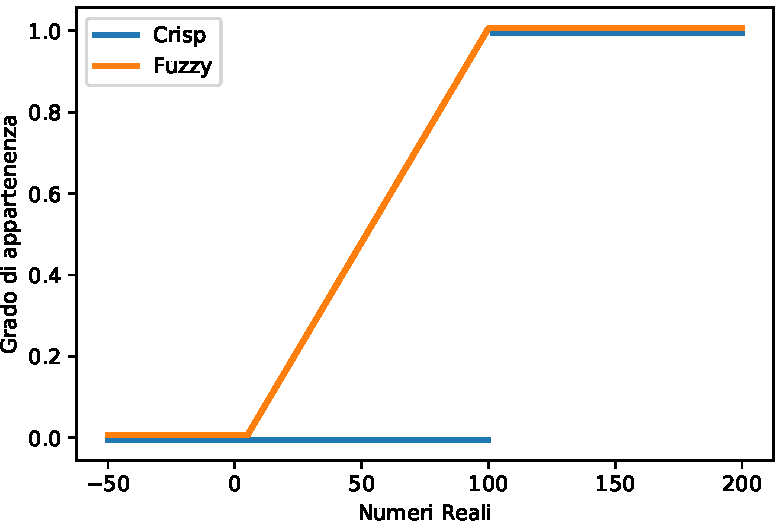
\includegraphics[scale=0.6]{figure/fuzzycrisp.pdf}
\caption{Grafico delle funzioni di appartenenza all'insieme ``Numeri molto più grandi di 1'' nelle versioni crisp e fuzzy \label{fuzzycrisp}}
\end{figure}
che meglio rappresenta il concetto di \textit{molto} più grande alla base della definizione dell'insieme $A$. La \figurename~\ref{fuzzycrisp} mostra una rappresentazione grafica di questa funzione di appartenenza, sovrapposta a un'analoga rappresentazione del concetto di appartenenza per un insieme \textit{crisp}, un insieme inteso nel senso classico del termine.\\
Nonostante l'appartenenza venga misurata con un numero compreso tra zero e uno, il concetto di appartenenza fuzzy non ha niente a che vedere con la probabilità di un elemento di appartenere ad un certo insieme e la logica fuzzy non ha niente a che vedere con la probabilità che coinvolge variabili casuali, non presenti nella logica fuzzy, e tratta di eventi e della loro possibilità di verificarsi. La \textit{fuzziness} è il risultato dell'imprecisione e dell'assenza di criteri chiari e ben definiti di appartenenza a un insieme.\\
Pertanto un insieme fuzzy è una collezione do oggetti con un grado non binario di appartenenza. Tale insieme è caratterizzato da una funzione che assegna a ogni oggetto un grado di appartenenza tra zero e uno, come formalmente indicato nella definizione seguente\cite{zadeh1965fuzzy}.
\begin{fuzzyset}
Sia $\Omega$ un insieme di punti in uno spazio, il cui generico elemento di $\Omega$ è denotato usando il simbolo $x$. Un \textit{insieme fuzzy} (o \textit{fuzzy set}) $A \subseteq \Omega$ è caratterizzato da una funzione di \textit{appartenenza} (o \textit{indicatrice}) $\mu_{A}(x)$ che associa ad ogni punto $x \in \Omega$ un valore reale nell'intervallo $[0,1]$, che rappresenta il \textit{grado di appartenenza} di $x$ a $A$.
\end{fuzzyset}
\begin{figure}[!h]
        \centering%
        \subfigure[Insieme delle persone giovani\label{giovani}]%
          {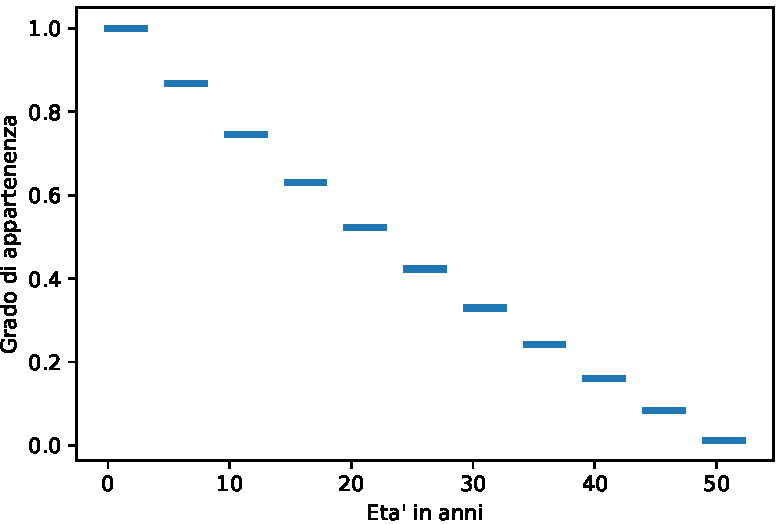
\includegraphics[scale=0.4]{figure/giovani.pdf}}\qquad\qquad
        \subfigure[Insieme delle bevande tiepide\label{tiepide}]%
          {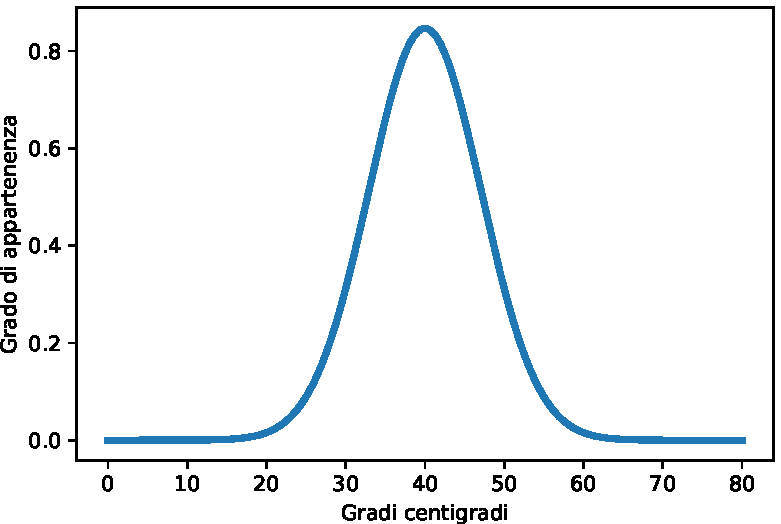
\includegraphics[scale=0.4]{figure/tiepide.pdf}}
          \caption{Alcuni esempi di fuzzy set con relativo grafico della funzione di appartenenza. Nella figura \figurename~\ref{giovani} l'insieme delle persone giovani è caratterizzato da una funzione \emph{non} continua rappresentata tramite un diagramma a barre. Nella figura \figurename~\ref{tiepide} l'insieme delle bevande tiepide è caratterizzato da una funzione di tipo unimodale.}
\end{figure}
\section{Operazioni tra insiemi fuzzy}
Sia per un insieme fuzzy, sia per un insieme del tipo ordinario, il grado di appartenenza zero ha il significato di \textit{non} appartenenza all'insieme e il grado di appartenenza 1 ha invece il significato di appartenenza. Gli insiemi fuzzy possono essere dunque visti come un'estensione degli insiemi crisp questi ultimi come un caso particolare di insiemi fuzzy la cui funzione di appartenenza è di tipo binario. Tutte le operazioni che si possono compiere con gli insiemi crisp sono estendibili agli insiemi fuzzy e tutte le definizioni fuzzy sono riconducibili a quelle crisp. Di seguito sono passate in rassegna le principali operazioni che coinvolgono degli insiemi, descrivendo come queste possano essere estese agli insiemi fuzzy.\\\\
\textbf{Insieme vuoto.} Un insieme fuzzy $A$ è vuoto se e solo se
\[ \mu_A(x) = 0 \; \forall \; x \in \Omega.\] 
\textbf{Uguaglianza.} Due insiemi fuzzy $A$ e $B$ sono uguali, scritto come $A=B$, se e solo se
\[ \mu_A(x) = \mu_B(x) \; \forall \; x \in \Omega.\] 
\textbf{Sottoinsiemi.} Un insieme fuzzy $A$ è sottoinsieme di un insieme fuzzy $B$, scritto come $A \subseteq B$, se e solo se
\[ \mu_A(x) \leq \mu_B(x) \; \forall \; x \in \Omega.\] 
\textbf{Complemento.} Il complemento di un fuzzy set $A$ è il fuzzy set $\bar{A}$, la cui funzione di appartenenza $\mu_{\bar{A}}$ è tale che
\[ \mu_{\bar{A}}(x) = 1-\mu_A(x) \; \forall \; x \in \Omega.\] 
\textbf{Unione.} L'unione tra un insieme fuzzy $A$ ed un insieme fuzzy $B$ è un insieme fuzzy $C$, scritto $C=A \cup B$, la cui funzione di appartenenza $\mu_C$ è tale che
\[ \mu_C(x) = \max[\mu_A(x), \mu_B(x)] \; \forall \; x \in \Omega\] 
\textbf{Intersezione.} L'intersezione tra un insieme fuzzy $A$ ed un insieme fuzzy $B$ è un insieme fuzzy $C$, scritto $C=A \cap B$, la cui funzione di appartenenza $\mu_C$ è tale che
\[ \mu_C(x) = \min[f_A(x), f_B(x)] \; \forall \; x \in \Omega.\] 
Va notato come queste estensioni non siano necessariamente uniche. Per esempio l'unione $A \cup B$ si può definire come il \textit{più piccolo} insieme fuzzy $C$ che contiene sia $A$ che $B$. Viceversa l'intersezione $A \cap B$ può essere definita come il \textit{più grande} insieme fuzzy $C$ che è contenuto sia in $A$ che in $B$. In entrambi i casi gli operatori $\cup$ e $\cap$ sono associativi. Infine due insiemi fuzzy sono \textit{disgiunti} se la loro intersezione è l'insieme vuoto.
\section{Fuzzy set di tipo 2}

\chapter{Support Vectors}
\section{Classificazione}
Classificare significa assegnare oggetti a classi secondo criteri di affinità. Un problema di classificazione consiste nella costruzione di una regola $f: \Omega \rightarrow Y$ che associa gli elementi del dominio $\Omega$ alle \textit{etichette} appartenenti al codominio $Y$ dove ogni diversa etichetta individua una diversa classe. L'insieme $\Omega$ tipicamente un sottoinsieme $\Omega \subseteq \mathbb{R}^d$. Il generico elemento di $\Omega$ è quindi un punto \textit{d}-dimensionale. Ciascuna delle \textit{d} dimensioni equivale a una specifica \textit{feature} della famiglia di oggetti $\Omega$. Nell'ambito del machine-learning il processo di costruzione della regola $f$ è detto \textit{apprendimento}. Durante la fase di apprendimento , un algoritmo visiona un insieme del tipo $T=\lbrace (x_0,y_0), (x_1,y_1), \cdots, (x_n,y_n) \rbrace$, dove la generica coppia $(x_i,y_i)$, con $x_i \in X \subseteq \Omega$ e $y_i \in Y$, è un esempio di classificazione corretta di $x_i$ con l'etichetta $y_i$, e ne estrae un criterio di classificazione generale per tutti i punti appartenenti a $\Omega$, cioè la funzione $f$. L'insieme $T$ prende il nome di \textit{training set}.\\
La notazione $x_i$ indica il primo elemento della \textit{i}-esima coppia appartenente ad un training set $T$. Mentre la notazione $x_{i}^{(j)}$ indica la \textit{j}-esima componente del vettore $x_i$. Quando la cardinalità dell'insieme di arrivo è $|Y|=2$, si parla di classificazione binaria. Per comodità di notazione e di calcolo da qui in poi verranno presentati esempi di classificazione binaria in cui l'insieme $Y$ delle possibili etichette è $Y=\lbrace-1,1\rbrace$.
\subsection{Percettrone}
Il percettrone \cite{rosenblatt1958perceptron} è un classificatore binario a soglia che assegna un oggetto $x \in \Omega$ alla classe ottenuta utilizzando la seguente regola:
\[
f_P(x)=
\begin{cases}
+1 & \textit{se } w \boldsymbol{\cdot} x \geq \theta, \\
-1 & \textit{se } w \boldsymbol{\cdot} x < \theta.
\end{cases}
\]
$w$ è un vettore di pesi, delle stesse dimensioni del vettore di input $x$, $\theta$ è la soglia discriminante nella classificazione di un punto e $\boldsymbol{\cdot}$ indica il prodotto scalare. Se la somma delle componenti del vettore input $x$ pesate secondo quelle del vettore $w$ supera una certa soglia $\theta$, il percettrone da un responso \textit{positivo}, altrimenti \textit{negativo}. L'iperpiano di equazione $w \boldsymbol{\cdot} x = \theta$ separa in $\Omega$ la classe positiva da quella negativa. La classificazione tramite percettrone è quindi applicabile con classi \textit{linearmente separabili} nello spazio di definizione. La fase di apprendimento dell' iperpiano $w \boldsymbol{\cdot} x = \theta$ consiste nell'aggiustare iterativamente i valori di $w$ fino a quando non si ottiene un iperpiano separatore corretto per il training set visionato, secondo una procedura simile a quella descritta nell'algoritmo \ref{iperpiano}.
\begin{algorithm}
\caption{Ricerca dell'iperpiano separatore}\label{iperpiano}
\begin{algorithmic}[1]
\State inizializzare $w$ con un vettore casuale
\While{esistono errori di classificazione}
	\State $i=0$
	\While{$i<|T|$}
		\State $y' = w \boldsymbol{\cdot} x_i - \theta$
		\If{$y' \cdot y < 0$} $w = w + \eta y x_i$ \EndIf
	\EndWhile
\EndWhile
\end{algorithmic}
\end{algorithm}
Si può dimostrare \cite{rosenblatt1958perceptron} che quando le due classi sono linearmente separabili, il punto 9 viene superato dopo un numero finito di iterazioni. In tal caso, l'iperpiano separatore è individuato da $w \boldsymbol{ \cdot} x = \theta$. In presenza di classi \textit{non} linearmente separabili il precedente algoritmo rimane bloccato in un loop infinito. Accettando di avere a che fare con classi non separabili l'algoritmo può essere modificato permettendo lo stop secondo alcuni criteri, per esempio eseguendo un numero fissato di cicli, oppure fermandosi quando il numero di classificazioni errate smette di variare al variare di $w$. L'istruzione 5 esegue l'aggiornamento di $w$, facendo in modo che il nuovo $w$ risulti spostato verso il vettore $x_i$ che è mal classificato in quel momento. Il parametro $\eta > 0$ definisce la misura dello spostamento e di conseguenza la velocità con cui $w$ si avvicina alla soluzione. Un $\eta$ troppo grande potrebbe portare a una situazione di loop infinito in cui $w$ continui ad aggiornarsi tra due valori, uno più grande, uno più piccolo della soluzione, o anche a far divergere $w$.\\
Nell'algoritmo \ref{iperpiano} la soglia $\theta$ è trattata come costante. È possibile permettere alla soglia di variare eliminandola di fatto dalla formalizzazione e aggiungendo una variabile in coda, come nuova dimensione, al vettore $w$. Aggiungendo agli esempi $x_i$ con lo stesso metodo il peso -1 il calcolo di $y'$ risulta analogo a quello del punto 3 e la soglia è in grado di variare come ogni altra singola componente di $w$.
\subsection{Macchine a vettori di supporto}
Una macchina a vettori di supporto, \textit{support vector machine}, o SVM in breve, ha come scopo non solo quello di trovare un iperpiano $w \boldsymbol{\cdot} x + b = 0$ che separi linearmente i dati, ma anche di fare in modo che l'iperpiano minimizzi l'errore durante la fase di classificazione di punti al di fuori dell'insieme di training. Questo iperpiano è quello posizionato alla stessa distanza da entrambe le classi. La distanza di una classe da un piano equivale alla minima distanza punto-piano misurata per ogni punto appartenente alla classe. Questa distanza viene definita \textit{margine}. Utilizzare l'iperpiano equidistante dalle classi per la discriminazione tra le due consente ai nuovi punti di scostarsi da quelli del training set ed essere comunque correttamente classificati. In questo modo tale spostamento può essere il più ampio possibile. In figura \ref{margine} la rappresentazione grafica di quanto scritto finora.
\begin{figure}[!h]
\centering
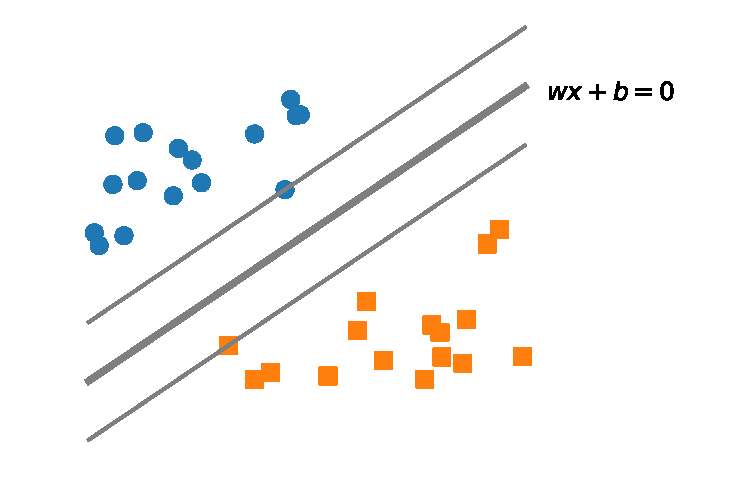
\includegraphics[scale=.6]{figure/margine.pdf}
\caption{Iperpiano separatore per due classi linearmente separabili in due dimensioni. In evidenza  i punti che si trovano alla minima distanza dall'iperpiano.  Il margine è individuato dalle rette più sottili.\label{margine}}
\end{figure}\\
La fase di apprendimento di SVM consiste nella massimizzazione del margine $\gamma$, variando i parametri $w$ e $b$, soggetta al vincolo che per ogni punto $x_i$, valga
\[
y_i(w\boldsymbol{\cdot}x_i + b) \geq \gamma.
\]
Indicando con $w^*$ e $b^*$ le soluzioni del precedente problema di massimizzazione sono individuati
\begin{itemize}
\item[]$w \boldsymbol{\cdot} x + b = 0$, l'iperpiano separatore.
\item[]$w \boldsymbol{\cdot} x + b = \gamma$, l'iperpiano contenente i punti appartenenti al margine positivo.
\item[]$w \boldsymbol{\cdot} x + b = -\gamma$, l'iperpiano contenente i punti appartenenti al margine negativo.
\end{itemize}
I punti che soddisfano l'equazione $w^* \boldsymbol{\cdot} x + b^* = \pm \gamma$, si trovano esattamente a distanza $\gamma$ dal separatore e si trovano sul confine delle loro classi. Tali punti prendono il nome di \textit{support vector} o \textit{vettori di supporto}. La figura \ref{supportvector} mette in evidenza i vettori di supporto per due classi linearmente separabili.\\
\begin{figure}[!h]
\centering
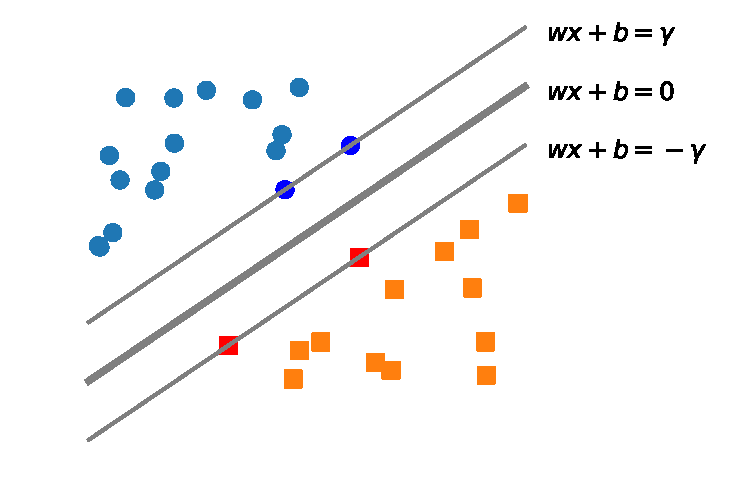
\includegraphics[scale=.6]{figure/supportvectors.pdf}
\caption{Support vectors per due classi linearmente separabili. Il valore di $\gamma$ è posto a 1 in accordo con il problema di normalizzazione dell'iperpiano. \label{supportvector}}
\end{figure}Scelta una coppia $(w^*, b^*)$ di soluzioni, è sempre possibile trovare una coppia $(kw^*, kb^*)$, per $k>1$, anch'essa soluzione, per cui è sempre vero che $k\gamma > \gamma$. In altre parole, $\gamma$ non può essere massimizzata. La soluzione a questo problema consiste nella normalizzazione del vettore $w$ costringendo $\gamma$ a essere multiplo del vettore unità $\dfrac{w}{\parallel w \parallel}$. Questo cambia il problema di ottimizzazione nella minimizzazione di $\parallel w \parallel$ soggetta al vincolo che per ogni punto $x_i$ valga
\[
y_i(w\boldsymbol{\cdot}x_i + b) \geq 1.
\]
Una volta determinati tali valori ottimali, la classificazione viene eseguita secondo la regola
\[
f_\mathrm{SVC}(x)=
\begin{cases}
+1 & \textit{se } w^* \boldsymbol{\cdot} x + b^* \geq 0, \\
-1 & \textit{se } w^* \boldsymbol{\cdot} x  + b^*< 0.
\end{cases}
\]
Va notato che il problema di minimizzazione di $\parallel w \parallel$ e quello di una qualsiasi funzione monotona di $\parallel w \parallel$ hanno le stesse soluzioni. Per comodità di derivazione e risoluzione normalmente si sceglie di costruire il problema di minimizzazione attorno alla funzione $f(\parallel w \parallel) = \dfrac{1}{2}\parallel w \parallel ^2$, trasformando il problema in minimizzare $\dfrac{1}{2}\parallel w \parallel ^2$ sotto i vincoli $ y_i(w\boldsymbol{\cdot}x_i + b) \geq 1 \; \forall \; x_i \in X$. Scrivere la lagrangiana
\[
L = \dfrac{1}{2}\parallel w\parallel ^2 - \sum_{i=1}^n \alpha_i [y_i(w \boldsymbol{\cdot} x_i +b -1)],
\]dove ogni $\alpha_i \geq 0$ è un moltiplicatore lagrangiano, permette di inglobare i vincoli nel problema. Differenziando $L$ per $w$ e per $b$ si ottiene
\begin{itemize}
\item[]$\dfrac{\partial L}{\partial w} = 0 \Longrightarrow w = \sum_{i=1}^n \alpha_i y_i x_i$,
\item[]$\dfrac{\partial L}{\partial b} = 0 \Longrightarrow \sum_{i=1}^n \alpha_i y_i = 0$.
\end{itemize}
Questi risultati, sostituiti a \ref{lagrange}, portano a quello che è definito \textit{problema duale}\cite{Fletcher}: massimizzare
\[
L_D = \sum_{i=1}^n \alpha_i -\dfrac{1}{2} \sum_{i,j}^n \alpha_i \alpha_j y_i y_j x_i \boldsymbol{\cdot} x_j,
\]
variando le nuove variabili $\alpha_i$ sotto i vincoli
\[
\alpha_i \geq 0 \; \forall i,
\]
\[
\sum_{i=1}^n \alpha_i y_i = 0.
\]
$w*$ è ricavabile da \ref{x}. L'introduzione delle nuove variabili $\alpha_i$ permette anche di avere informazioni riguardanti i support vector. Ad $\alpha_i > 0$ corrisponde $x_i$ tale che $x_i$ è un vettore di supporto. A questo punto $b^*$ è la soluzione dell'equazione $y_i(w^* \boldsymbol{\cdot} x_i + b)= 1$ dove $x_i$ è uno tra i vettori di supporto individuati. 
\subsection{Kernel Trick}
Quello di utilizzare uno, o più, piani separatori è un buon metodo di classificazione in presenza di dati linearmente separabili. Al contrario, in presenza di dati non linearmente separabili qualsiasi scelta per la coppia $(w^*, b*)$ produce un iperpiano che mal classifica almeno un elemento del training set. La figura \ref{nonseparabili} rappresenta graficamente una di queste situazioni
\begin{figure}[!h]
\centering
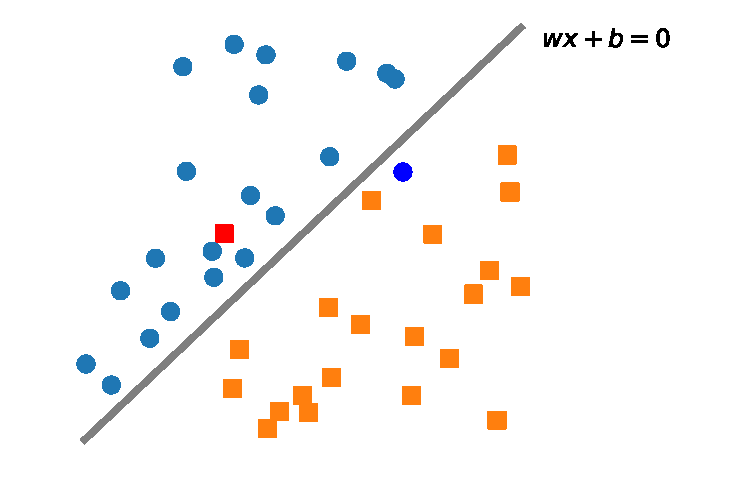
\includegraphics[scale=.6]{figure/nonseparabili.pdf}
\caption{Esempio in due dimensioni di classi non linearmente separabili. In evidenza i punti male classificati. \label{nonseparabili}}
\end{figure}
Una delle possibili soluzioni a questa situazione è quella di trasformare i dati in modo che siano linearmente separabili utilizzando il \textit{kernel trick}. L'idea che sta dietro al \textit{trucco} è quella che punti \textit{d}-dimensionali, non linearmente separabili in \textit{d} dimensioni, potrebbero esserlo se trasportati in uno spazio a maggiore dimensionalità. Una funzione $\phi: \mathbb{R}^d \rightarrow \mathbb{R}^D$, per $D > d$, che trasporta punti in uno spazio a maggiore dimensionalità aggiungendo le feature mancanti come funzione di quelle originali è chiamata \textit{mapping}. Per sortire l'effetto di produrre dati linearmente separabili un mapping deve poter proiettare in porzioni differenti dello spazio punti appartenenti a differenti classi.\\\\
\textbf{Esempio 1.} Dato il training set $T_1=\lbrace (1,a),(-2,a),(3,b),(-3,b),(-4,b), \linebreak (-1,a),(4,b),(2,a) \rbrace$ dove $X = \lbrace x \in \mathbb{N}^1 | -5 < x < 5 \rbrace$ e $Y=\lbrace a,b \rbrace$, le due differenti classi risultano non linearmente separabili sulla retta dei reali, come osservabile in \figurename~\ref{mapping12}. Il mapping $\phi_1(x)=(x,x^2)$ proietta verso l'alto gli $x \in X$ con modulo maggiore, rendendo il training set linearmente separabile nelle due dimensioni, osservabile in \ref{mapping12}.
\begin{figure}[!h]
        \centering%
        \subfigure[Grafico unidimensionale del training set\label{mapping11}]%
          {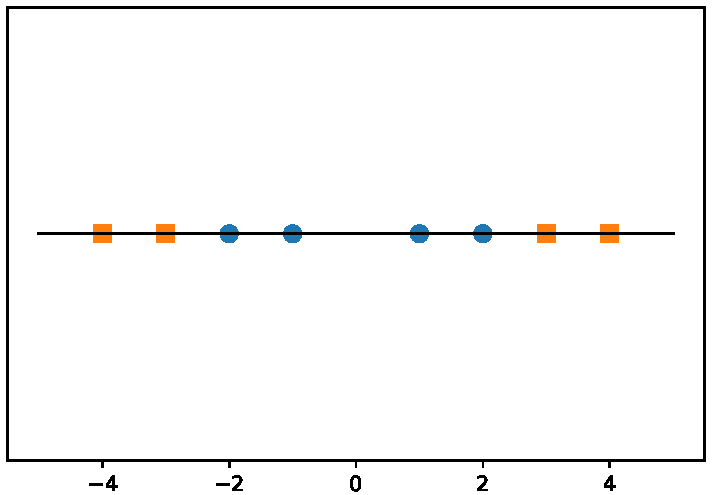
\includegraphics[scale=0.4]{figure/mapping11.pdf}}\qquad\qquad
        \subfigure[Grafico dell'immagine training set nello spazio bidimensionale creato dal mapping $\phi_1$\label{mapping12}]%
          {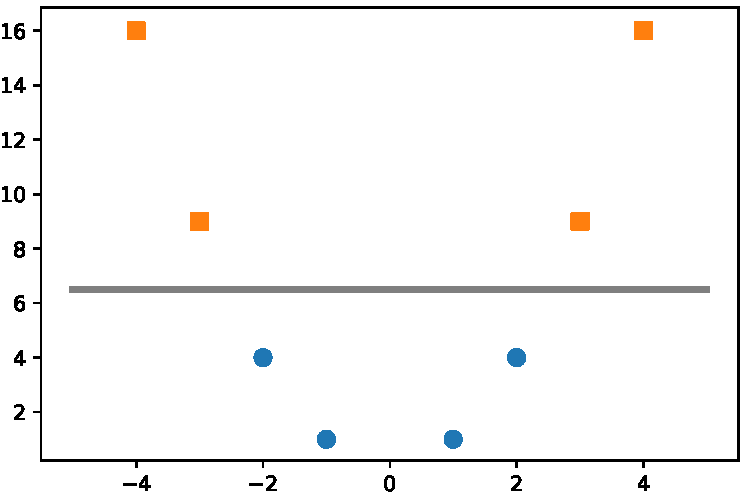
\includegraphics[scale=0.4]{figure/mapping12.pdf}}
          \caption{Grafici del training set $T_1$ nello spazio originale e in quello mappato. Nella \figurename~\ref{mapping12} in evidenza l'iperpiano separatore delle classi.}
\end{figure}
\linebreak
\textbf{Esempio 2.} Dato il training set $T_2=\lbrace [(0;3),a], [(3;0),a], [(1;2),b], \linebreak (2;1),b], [(\dfrac{3}{2};0),a], [(0;\dfrac{3}{2}),a], [(1;1),b], [(2;2),b] \rbrace$, con $X \subset \mathbb{R}^2$, in cui le classi $a, b \in Y$ non sono linearmente separabili (\figurename~\ref{mapping21}). la trasformazione $\phi_2(x,y)=(x,y,xy)$ produce valori bassi nella terza dimensione per i punti etichettati $a$, valori alti per i punti etichettati $b$, rendendo l'immagine di $X$ linearmente separabile nello spazio tridimensionale (\figurename~\ref{mapping22}).
\begin{figure}[!h]
        \centering%
        \subfigure[Grafico bidimensionale del training set\label{mapping21}]%
          {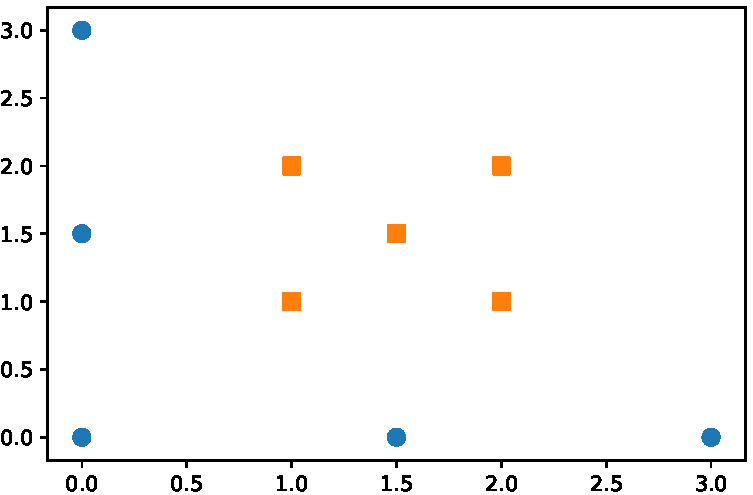
\includegraphics[scale=0.4]{figure/mapping21.pdf}}\qquad\qquad
        \subfigure[Grafico dell'immagine del training set nello spazio tridimensionale creato dal mapping $\phi_2$\label{mapping22}]%
          {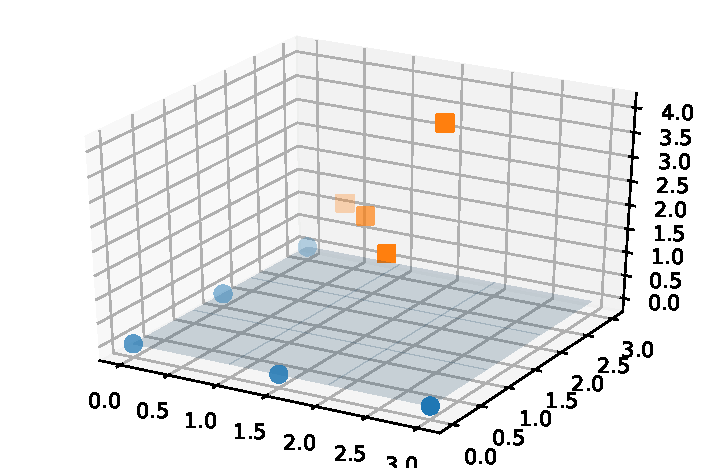
\includegraphics[scale=0.4]{figure/mapping22.pdf}}
          \caption{Grafici del training set $T_2$ nello spazio originale e in quello mappato. Nella \figurename~\ref{mapping22} in evidenza l'iperpiano separatore delle classi.}
\end{figure}
\linebreak
In questo caso la regola di classificazione diventa quindi
\[
f_K(x)=
\begin{cases}
+1 & \textit{se } w^* \boldsymbol{\cdot} \phi(x) + b^* \geq 0, \\
-1 & \textit{se } w^* \boldsymbol{\cdot} \phi(x)  + b^*< 0.
\end{cases}
\]
La denominazione \textit{kernel trick} deriva dal fatto che il trucco è utilizzato in coppia con funzioni denominate \textit{kernel function}\cite{giannelli}. Considerato un mapping $\phi$, una kernel function $K$ è definita in modo tale che sia sempre valido
\[
K(x_i,x_j) = \phi(x_i) \boldsymbol{\cdot} \phi{x_j}.
\]
In questo modo, conoscendo $K$, è possibile calcolare il prodotto scalare tra due elementi appartenenti all'insieme ad alta dimensionalità senza dover effettivamente calcolare i mapping corrispondenti. Così facendo la \ref{duale} può essere riscritta in questo modo:
\[
L_D = \sum_{i=1}^n \alpha_i -\dfrac{1}{2} \sum_{i,j}^n \alpha_i \alpha_j y_i y_j K(x_i,x_j).
\]
\subsection{Dati non separabili}

\section{1-SVM}

\section{Clustering}

\bibliographystyle{unsrt}
\bibliography{tesi.bib}
\end{document}